%************************************************
\chapter{About Dorel Industries}
\label{chp:about}
%************************************************

In 1962, Leo Schwartz founded "Dorel Co. Ltd" in Quebec, and began producing juvenile products.  It was not until 1962 that "Dorel Co. LTD" became "Dorel Industries", following a merger with Ridgewood Industries (a furniture manufacturing company).  Since then, the company has continued to grow primarily through acquisitions, eventually branching out to the recreational and leisure markets by acquiring Schwinn and Cannondale


\section{Recent Strategic Moves (2013)}
\begin{itemize}
  \item Dorel began a massive share buyback plan in order to raise its market value.
  \item The company acquired a 70% controlling interest in Caloi (a major brazilian bicycle manufacturer).  This acquisition is intended to help Dorel expand into Latin America, as Caloi is the number one bicycle brand in the region.
  \item Dorel’s assembly and testing facilities located in Bedford, PA are being shut down and relocated overseas in an effort to reduce expenses.
\end{itemize}


%************************************************
\chapter{Business Overview}
\label{chp:overview}
%************************************************


\section{Business Definition}

Dorel Industries has a diverse business definition.   Dorel makes high quality furniture, juvenile and recreational products for consumers who emphasize quality and durable products.  Dorel’s technologies include ready-to-assemble furniture, high quality and durable bicycles as well as safe and reliable baby products.

As you can see in the below figure, Dorel’s business is comprised of very distinct products amongst distinct markets. Dorel’s main products include furniture, bicycles and baby products.  These products relate to Dorel’s business units.   In term’s of Dorel’s target markets, United States is a very important market. However, due to the US economy downturn, this has made Dorel focus on extending their business internationally.  Lastly, the technology that Dorel institutes is one of outsourcing manufacture of their products, in order to be able to compete on price, specifically for their home furnishings business unit.

One, of many, issues with this business definition is there does not appear to be synergies amongst either the manufacture of the products, the products themselves, nor the target markets of each product. As part of our recommendation, Dorel would benefit from finding a way to have more synergies amongst their most important products. 

\begin{itemize}        	
  \item Products
    \begin{itemize}
      \item Furniture
      \item Bicycles
      \item Baby products/accessories
    \end{itemize}
  \item Markets (respectively)
    \begin{itemize}     
      \item North American retail chains
      \item Mass merchant / Independent Bike Dealer (IBD) network
      \item US and International retail chains
    \end{itemize}
  \item Technology
    \begin{itemize}     
      \item Ready-to-assemble furniture
      \item High Quality products
      \item Safe and durable juvenile products
    \end{itemize}
\end{itemize}





\section{Business Unit Breakdown}
Dore’s business is comprised of 3 distinct business units; Juvenile, Home Furnishings and Recreational/Leisure.  These 3 business units drove 2012 revenue of $2.49 Billion, as well as $583 Million in gross profit. A breakdown of each business unit follows.

\subsection{Juvenile}
The typographical style achieved with \arsclassica{} differs from ClassicThesis in the following points:
\begin{itemize}
\item use of Iwona\index{Iwona} font, by Janusz M.~Nowacki, for the titles of the sectioning units of the document (chapters, sections, subsections, sub-subsections, paragraphs and subparagraphs), for the labels of description lists, for the headlines and the label of the captions (\classicthesis{} does not use any sans serif font);
\item customized chapter numbers;
\item semi-transparent headlines; the headlines are separated from the page number by a small rule;
\item captions with labels in boldface (\classicthesis{} does not use any boldface font);
\item itemize lists with semi-transparent bullets.
\end{itemize}

The \arsclassica{} package is designed  to provide a ready-to-use typographical style: therefore it has no loading option and it is \emph{not} configurable or customizable in any way. If you change the previous settings, you will risk to destroy the balance of the style, so it is \emph{highly recommended} to keep them unchanged.

One of the principles of \LaTeX{} is that it allows the author to take no interest in the typographical questions, permitting him to focus only the structure and the contents of the document. This fact should always be taken in consideration: using a style written by others, the user accepts all the typographical settings chosen for him by the author of the style, and he is not forced to study typography to fix the layout of his publications. This is the case of \arsclassica{} too: if you change its settings, you will deny this philosophy and, consequently, you must study (a lot of) typography to achieve acceptable results. 

The style achieved with \arsclassica{} is \emph{not} therefore configurable or customizable. The typographical style is something of very personal: if you like the package and find attractive the idea to take no interest in the problem of the style definition, then you will use \arsclassica{} with satisfaction; otherwise, if you have different needs or you are not satisfied with the layout of the package, then you should try other classes or packages, even building your own style.



\section{New commands}

The package offers the \cmdname{ctLaTeX}, \cmdname{ctLaTeXe} and \cmdname{ctTeX} commands, which allow to reproduce respectively the \LaTeX, \LaTeXe{} and \TeX{} logos correctly written in Iwona.\index{Iwona}






\section{Examples}

\begin{figure}
\centering
\subfloat[Asia personas duo.]
{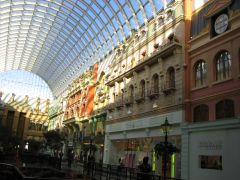
\includegraphics[width=.45\columnwidth]{Example_1}} \quad
\subfloat[Pan ma signo.]
{\label{fig:example-b}%
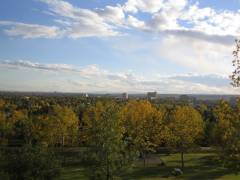
\includegraphics[width=.45\columnwidth]{Example_2}} \\
\subfloat[Methodicamente o uno.]
{
\includegraphics[width=.45\columnwidth]{Example_3}} \quad
\subfloat[Titulo debitas.]
{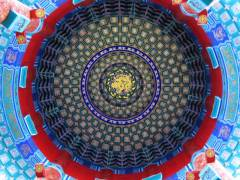
\includegraphics[width=.45\columnwidth]{Example_4}}
\caption[Tu duo titulo debitas latente.]{Tu duo titulo debitas
latente.}\label{fig:example}
\end{figure}

Note: The content of this chapter is just some dummy text. It is not a real language.

Lorem ipsum dolor sit amet, consectetuer adipiscing elit. Ut purus elit, vestibulum ut, placerat ac, adipiscing vitae, felis. Curabitur dictum gravida mauris. Nam arcu libero, nonummy eget, consectetuer id, vulputate a, magna. Donec vehicula augue eu neque.

\subsection*{A subsection}
\lipsum[2]

\subsubsection*{A sub-subsection}
\lipsum[3]

\paragraph{A paragraph} Lorem ipsum dolor sit amet, consectetuer adipiscing elit. Ut purus elit, vestibulum ut, placerat ac, adipiscing vitae, felis. Curabitur dictum gravida mauris. Nam arcu libero, nonummy eget, consectetuer id, vulputate a, magna.

\bigskip

\lipsum[2]

\begin{description}
\item[Mane] Lorem ipsum dolor sit amet, consectetuer adipiscing elit. 
\item[Tekel] Ut purus elit, vestibulum ut, placerat ac, adipiscing vitae, felis. Curabitur dictum gravida mauris.
\item[Fares] Nam arcu libero, nonummy eget, consectetuer 
id, vulputate a, magna.
\end{description}

\begin{table}
\caption[Lorem ipsum dolor.]{Lorem ipsum dolor sit amet.}
\centering
\begin{tabular}{cc}
\toprule
$p$ & $\lnot p$ \\ 
\midrule
V   & F \\ 
F   & V \\
\bottomrule 
\end{tabular}
\end{table}

\lipsum[1]




